\documentclass[12pt,reqno, twoside]{amsbook}
%%%%%%%%%%%%%%%%%%%%%%%%%%%%%%%%%%%%%%%%%%%%%%%%%%%%%%%%%%%%%%%%%%%%%%%%%%%%%%%%%%%%%%%%%%%%%%%%%%%%%%%%%%%%%%%%%%%%%%%%%%%%%%%%%%%%%%%%%%%%%%%%%%%%%%%%%%%%%%%%%%%%%%%%%%%%%%%%%%%%%%%%%%%%%%%%%%%%%%%%%%%%%%%%%%%%%%%%%%%%%%%%%%%%%%%%%%%%%%%%%%%%%%%%%%%%
\usepackage{eurosym}
\usepackage{amsmath}
\usepackage{amssymb}
\usepackage{amsfonts}
\usepackage{chngcntr}
\usepackage{graphicx}
\usepackage{csquotes}
\usepackage{subcaption}
\usepackage[a4paper, margin=2.5cm]{geometry}
\usepackage[english]{babel}
\usepackage{fancyhdr}
\usepackage{titlesec}
\usepackage{enumitem}
\usepackage{etoolbox}
\usepackage{booktabs}
\usepackage{lscape}
\usepackage{tabularx}
\usepackage{rotating}    % for sidewaystable
\usepackage{adjustbox}   % to scale table content
\usepackage{afterpage}

\usepackage[labelfont=normalfont,textfont=normalfont]{caption}
\usepackage[table]{xcolor}
\usepackage[acronym]{glossaries}
\makeglossaries
\usepackage[style=apa,backend=biber]{biblatex}
\addbibresource{references.bib}
\usepackage{svg}
\usepackage[hidelinks]{hyperref}
\hypersetup{
    linktoc=all,     %set to all if you want both sections and subsections linked
}
\usepackage{times}
\usepackage[onehalfspacing]{setspace}
\setlength{\parindent}{0.7cm}
\setlength{\parskip}{0pt}
\titlespacing{\section}{0pt}{1.5\baselineskip}{\baselineskip} % (left, before, after)
\titlespacing{\subsection}{0pt}{\baselineskip}{\baselineskip}
\titlespacing{\subsubsection}{0pt}{\baselineskip}{\baselineskip}
\fancyfoot[LE,RO]{\thepage} % Esquerda nas pares, direita nas ímpares
\setlength{\footskip}{1.25cm} % Distância ao fundo da página



% you may need to uncomment the command below if you use eps format for figures
%\usepackage{epstopdf}


\makeatletter
    \def\section{\@startsection{section}{1}%
      \z@{.5\linespacing\@plus.7\linespacing}{.25\linespacing}%
      {\normalfont\bfseries\flushleft}}
    \def\subsection{\@startsection{subsection}{2}%
      \z@{.5\linespacing\@plus.7\linespacing}{.25\linespacing}%
      {\normalfont\bfseries\flushleft}}
    \def\subsubsection{\@startsection{subsubsection}{3}%
      \z@{.5\linespacing\@plus.7\linespacing}{.25\linespacing}%
      {\normalfont\bfseries\flushleft}}

\makeatother
\setcounter{MaxMatrixCols}{10}

\providecommand{\U}[1]{\protect\rule{.1in}{.1in}}
\theoremstyle{plain}
\newtheorem{acknowledgement}{Acknowledgement}
\newtheorem{algorithm}{Algorithm}[chapter]
\newtheorem{axiom}{Axiom}[chapter]
\newtheorem{case}{Case}[chapter]
\newtheorem{claim}{Claim}[chapter]
\newtheorem{conclusion}{Conclusion}[chapter]
\newtheorem{condition}{Condition}[chapter]
\newtheorem{conjecture}{Conjecture}[chapter]
\newtheorem{corollary}{Corollary}[chapter]
\newtheorem{criterion}{Criterion}[chapter]
\newtheorem{definition}{Definition}[chapter]
\newtheorem{example}{Example}[chapter]
\newtheorem{exercise}{Exercise}[chapter]
\newtheorem{lemma}{Lemma}[chapter]
\newtheorem{notation}{Notation}[chapter]
\newtheorem{problem}{Problem}[chapter]
\newtheorem{proposition}{Proposition}[chapter]
\newtheorem{remark}{Remark}[chapter]
\newtheorem{solution}{Solution}[chapter]
\newtheorem{summary}{Summary}[chapter]
\newtheorem{theorem}{Theorem}[chapter]
\numberwithin{equation}{chapter}

\newcommand{\tabref}[1]{\textbf{Table~\ref{#1}}} 
\newcommand{\figref}[1]{\textbf{Figure~\ref{#1}}}
\counterwithout{figure}{chapter}
\counterwithout{table}{chapter}
\renewcommand{\thefigure}{\arabic{figure}}

\newenvironment{dedication}
  {%\clearpage           % we want a new page
   \thispagestyle{empty}% no header and footer
   \vspace*{\stretch{1}}% some space at the top
   \itshape             % the text is in italics
   \raggedleft          % flush to the right margin
  }
  {\par % end the paragraph
   \vspace{\stretch{3}} % space at bottom is three times that at the top
   %\clearpage           % finish off the page
  }
  \numberwithin{section}{chapter}
\fancyhead{}
\fancyfoot{}
\pagestyle{fancy}
\fancyfoot[LE,RO]{\thepage}

\makeatletter
\def\ps@plain{\ps@empty
 \def\@evenfoot{%
   \normalfont\scriptsize
   \rlap{\thepage}\hfil
   }%
 \def\@oddfoot{%
   \normalfont\scriptsize \hfil
   \llap{\thepage}}%
}
\makeatother
\renewcommand{\headrulewidth}{0pt}
\renewcommand{\footrulewidth}{0pt}

\newglossarystyle{glostable}
{%
    \renewenvironment{theglossary}
    {
        \begin{longtable}{|p{0.25\textwidth}|p{0.025\textwidth}|p{0.7\textwidth}|}
    }
    { \end{longtable} }

    \renewcommand*{\glossaryheader}
    {
        \hline
        \textbf{Symbol} & - & \textbf{Description} \\
        \hline
    }

    \renewcommand*{\glsgroupheading}[1]{}
    \renewcommand*{\glsgroupskip}{}
    \renewcommand{\glossentry}[2]
    {
        \glossentryname{##1} & - & \glossentrydesc{##1} \\
        \hline

    }
    \renewcommand*{\subglossentry}[3]{}
}

\begin{document}
\begin{titlepage}
    \raggedright
    
\includegraphics[width=0.4\textwidth]{assets/logo_iscte_ista.png} \\[1cm]
    
    \Large
    \textbf{\LARGE How Requirement Gathering influences Technical Debt and Quality in Software Development} \\[0.5cm]

    Master's in Computer Science and Business Management \\[2cm]
    
    Gonçalo Gonçalves Miranda \\[0.5cm]
    
    
    \raggedright
    Supervisor(s): TBD
    %PhD Rúben Filipe de Sousa Pereira, 
    %Assistant Professor, ISCTE-IUL 

    \vfill
    \centering
    \large
    ISCTE – Instituto Universitário de Lisboa \\
    \centering
    June, 2025
\end{titlepage}

\clearpage
\thispagestyle{empty}
\null
\frontmatter
\addtocontents{toc}{\setcounter{tocdepth}{3}    % include subsubsections in the ToC
\setcounter{secnumdepth}{3} % (optional) number subsubsections as well
}


\chapter*{Acknowledgement}

Write here the acknowledgments and grants, if any

\chapter*{Abstract}

In software engineering, the quality of Requirements Engineering (RE) is a key factor when predicting long-term success and sustainability of software systems. Requirements are the basis for any decision in the project, wether it is related to design, implementation, or maintenance. However, in practice, requirements are often incomplete, ambiguous, or unstable. These conditions provide a breeding ground to what is known as Requirements-Related Technical Debt (RTD). RTD captures the trade-offs made during the requirements phase that lead to architectural, functional, or documentation failures, which lead to increased maintenance costs, reduced adaptability, and long-term quality degradation.

While the general concept of Technical Debt (TD) has been thoroughly studied, the influence of requirement-related factors remains underdeveloped in the particular context of big corporations, where AGILE and fast-paced development environments are predominant and where decisions made under pressure or with little stakeholder involvement can silently build up as debt, with consequences that may only be detected down the line. Despite existing recommendations to neutralize such problems, the industry still suffers to consistently identify, track, and prevent RTD before it negatively impacts software evolution.

In order to tackle this gap, this research combines a Systematic Literature Review (SLR) of 30 publications with a case study elaborated in cooperation with a software company. The purpose is to consolidates existing work on RTD causes and mitigation approaches, and to validate these findings through empirical investigation. By doing this, the research aims to yield practical insights and theoretical clarity to support more resilient and sustainable RE practices.



\tableofcontents

\listoffigures
\listoftables

%Acronyms
\newacronym{slr}{SLR}{Systematic Literature Review}
\newacronym{mlr}{MLR}{Multivocal Literature Review}
\newacronym[description={Requirement Engineering}]{re}{RE}{requirement engineering}
\newacronym[description={Quality Requirements}]{qr}{QRs}{quality requirements}
\newacronym[description={Technical Debt}]{td}{TD}{technical debt}
\newacronym[description={Requirements-related Technical Debt}]{rtd}{RTD}{requirements-related technical debt}
\newacronym[description={Software Quality}]{sq}{SQ}{software quality}
\newacronym[description=Non-Functional Requirements]{nfr}{NFRs}{non-functional requirements}
\newacronym[description=Functional Requirements]{fr}{FRs}{functional requirements}
\newacronym{satd}{SATD}{Self-Admitted Technical Debt}
\newacronym{dsr}{DSR}{Design Science Research}
\newacronym{csr}{CSR}{Case Study Research}


\printglossary[type=\acronymtype,style=glostable,title={List of Acronyms}]

\mainmatter

\hyphenation{wri-te he-re pro-per hy-phe-ni-za-tion
}%

\setcounter{page}{1} \pagenumbering{arabic}

\chapter{Introduction}
\noindent As modern software systems increase in complexity and scale, the difficulty of maintaining stakeholders expectations aligned with system behavior also becomes more difficult and consequential, while also being more critical than ever \parencite{Venters2023}. Alongside that, both the quality and sustainability of a system's architectures heavily rely on early development life-cycle activities, with a huge focus on the quality of the \gls{re} process \parencite{Rios2019}. According to \textcite{Behutiye2022}, the robustness of this process must match the system's complexity, in order to ensure the system remains maintainable, adaptable and aligned with the long-term vision of the quality goals of the project. According both to \textcite{Behutiye2022,Melo2022}, this means the rigor, clarity, and completeness of the captured requirements influence not only the short-term development process but also the system's ability to progressively adapt to different contexts and new demands. Failing to attentively perform the activities related to this early phase of software engineering increases the likelihood of accumulated architectural and design flaws, paves the way for \gls{td}.


Although awareness of the risk incomplete, unstable or ambiguous requirements pose to a project is rising, many continue to suffer due to this factor, particularly in fast-paced environments where adaptability are prioritized over documentation and long-term planning, such as contexts related to AGILE and startups \parencite{Behutiye2022, Gupta2020}. Though AGILE methods may be beneficial for swift delivery and user-centric development, they often tend to undermine \gls{nfr} and a solid architectural design, which contributes to challenges in the long run, such as the need to refactor certain parts of the system or even quality degradation \parencite{Snoeck2022}, being the dynamic between short-term delivery goals and long-term software robustness becomes evident in cases where requirements deviate halfway through development or are under-specified.

Research in \gls{rtd} - which is one of the most common types of \gls{td}, according to \textcite{Wattanakriengkrai2018} - unveils that decisions made under uncertainty or pressure tend to output “quick fixes” that accumulate over time and hinder future changes, testing, or scale, as stated by \textcite{Melo2022}. In theory, these trade-offs are not inherently harmful, as they can be useful tools when correctly managed. However, in practice, \gls{rtd} is usually left unidentified or undocumented during the requirements phase, resulting in developer teams that are oblivious to the existence of such issues, until they cripple development progress, as documentation regarding \gls{qr} is usually less of a priority for development teams, regardless of the potential problems this is likely to cause in the long-term, according to  \textcite{Behutiye2022}.

The risk introduced by poor \gls{re} is particularly alarming in organizations that rely on swiftly composed or distributed teams. Due to this, this study aims to explore the influence of requirement gathering practices on the accumulation of \gls{td} and the quality of software outputs, while exploring what are the most common causes of \gls{rtd} and how they can be identified and correctly mitigated in a real world environment. 

\chapter{Related Work}
\section{Systematic Literature Review}
\noindent In order to summarize all current relevant academic knowledge regarding the topic subject to research, to identify research gaps and to indicate new areas for posterior investigation, this study was conducted as a \gls{slr} and followed the guidelines defined by \textcite{Kitchenham2007}, that divides the research into 3 different stages: the review planning, the review conduction, and the review report. As per the authors, a systematic approach is predefined using a review protocol that creates research questions and the methods used in the review, in order to target such questions. This allows for the study to be repeatable, which improves its transparency and enables any reader to assess a study's rigor and integrity \parencite{Kitchenham2007}.

\begin{figure}[htbp]
    \centering
    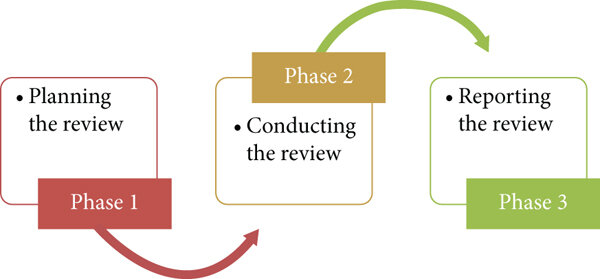
\includegraphics[width=0.7\textwidth]{assets/slr_phases.png} % make sure the image is in the same directory
    \caption{\gls{slr} Phases}
    \label{fig:slr_phases}
\end{figure}

\subsection{Review Planning Stage}
\noindent This section refers to the \gls{slr} methodology's first stage, where the rationale for conducting the 
review should be outlined, as well as the research questions, and where the review protocol is defined.
\subsubsection{Review Motivation}
\noindent Despite growing awareness of \gls{td} in software engineering, the impact of \gls{re} on its mitigation and accumulation remains underexplored. Unreliable requirements are often mentions as key actors to \gls{rtd}, mainly in environments where  documentation and \gls{qr} are often de-prioritized, such as AGILE and fast-paced development environments \parencite{Behutiye2022}. \textcite{Melo2022} states that, while causes and metrics for \gls{rtd} have been already draft by some studies, current work lacks a systematic and comprehensive compilation of how these issues are generated, as well as their impact on long-lasting product quality, and how they can be addressed correctly. Case studies that concern both small and large projects reveal that poor requirement gathering techniques can lead to extensive refactoring due to product misalignment with client expectations and to increased maintenance costs, indicators that are highly correlated with \gls{td} \parencite{Gupta2020}. This \gls{slr} is produced based on the need to clarify the connection between deficient \gls{re} and \gls{td}, to understand their long-term effects on \gls{sq}, and to identify ways to predict and mitigate \gls{rtd} in heterogeneous development contexts.
\subsubsection{Research Questions}

\noindent The focus of this review is to address the following questions:\par
\hspace*{\linewidth}\par
\noindent\textbf{RQ.1}: How do incomplete or evolving requirements contribute to the accumulation of \gls{td} in software development projects?\par
\hspace*{\linewidth}\par
\noindent\textbf{RQ.2}: What is the relationship between the quality of requirement gathering practices and software product quality outcomes over time?\par
\hspace*{\linewidth}\par
\noindent\textbf{RQ.3}: Which requirement-related factors most commonly lead to \gls{td}, and how are they identified and mitigated in practice?\par
\hspace*{\linewidth}\par
\noindent\textbf{RQ.4}: 
What RE process is most commonly linked to \gls{td}, and how can they improve to mitigate it?\par
\hspace*{\linewidth}\par
\noindent\textbf{RQ.5}: 
How do different project contexts and team structures affect the emergence or management of RTD?\par

\subsubsection{Review Protocol}
\noindent The databases considered for the search are SCOPUS\footnote{\url{https://www.scopus.com/}}, the ACM Digital Library\footnote{\url{https://dl.acm.org/}}, and the IEEE Xplore Digital Library\footnote{\url{https://ieeexplore.ieee.org/Xplore/home.jsp}} . 

\subsection{Review Conducting Stage}
\noindent This section represents the second stage in the \gls{slr} methodology, where the protocol's application is described. The analysis of the extracted data also occurs during this stage.
\subsubsection{Research Identification}
\noindent Starting from this study's research question, the necessary keywords to perform the research were extracted in order to generate an insightful search string, as shown in \tabref{tab:slr_keywords_and_search_string}.

\begin{table}[htbp]
    \centering
    \begin{tabular}{|>{\columncolor{gray!30}}c|c|}
        \hline
        Keywords & Technical Debt, Requirements, Software \\
        \hline
        Search String & "Technical Debt" AND "Requirements" AND "Software" \\
        \hline
    \end{tabular}
    \caption{SLR Keywords and Search string}
    \label{tab:slr_keywords_and_search_string}
\end{table}

\subsubsection{Study Selection}
\noindent For this study, 7 filters where used to thin down the search result, listed on \tabref{tab:filters}.
\clearpage
\begin{table}[htbp]
    \centering
    \begin{tabular}{|c|c|}
        \hline
        \rowcolor{gray!30}
        ID & Filter \\
        \hline
        1 & Title, Abstract or Keywords \\
        \hline
        2 & 2018-2025 \\
        \hline
        3 & English \\
        \hline
        4 & Articles, Conference Papers, Short Papers, Reviews and Conference Reviews \\
        \hline
        5 & 15 or more Citations \\
        \hline
        6 & Manual \\ 
        \hline
        7 & Backward Snowballing Search \\ 
        \hline
    \end{tabular}
    \caption{Search Filters}
    \label{tab:filters}
\end{table}

\noindent The research process was commenced with an initial, filter-less search of the selected search string across the 3 selected databases, which provided an output of 4408 results. Then, the first filter was introduced, "Title, Abstract or Keywords," which enabled a reduction in the number of studies to 295, followed by the 
application of the filter "2018-2025," that reduced the number of studies to be considered to 203. Afterwards, the third filter, "English", was applied, subtracting 5 more studies from the current pool, bringing it down to 198. After this, the "Articles, Conference Papers, Short Papers, Reviews and Conference Reviews" filter was applied, thinning down the possible studies to 151. However, the biggest decrease in number of articles was introduced by the fifth filter, "15 or more Citations", that downsized the study pool to only 29. Subsequently, a manual reading of all the studies allowed to both filter duplicate results and to select only relevant studies. With this, there was a reduction of 5 more studies, bringing the number of selected studies down to 25. Finally, this reading also enabled the application of the seventh filter: the "Backward Snowballing Search", which was based on the relevance of the studies and their citations. Only studies that met prior filters and acceptance criteria were selected, resulting in a definitive pool size of 30 articles, which were considered the most relevant studies, with this research's goal in mind. Besides this, 2 articles were selected to introduce both the \gls{slr} and the research methodology in use.
\tabref{tab:filtration_process} and \figref{fig:slr_search_filtration_diagram}, synthesize the process of the selection of the studies.

\begin{table}[htbp]
    \centering
    \resizebox{\textwidth}{!}{%
    \begin{tabular}{|c|c|c|c|c|c|c|c|c|}
        \hline
        \rowcolor{gray!30}
        Database & No Filter & Filter 1 & Filter 2 & Filter 3 & Filter 4 & Filter 5 & Filter 6 & Filter 7 \\
        \hline
        SCOPUS & 1765 & 182 & 132 & 127 & 126 & 22 & 19 & 4\\
        \hline
        IEEE Xplore Digital & 1705 & 86 & 53 & 53 & 8 & 4 & 3 & 0 \\
        \hline
        ACM Digital Library & 938 & 27 & 18 & 18 & 17 & 3 & 3 & 1 \\
        \hline
        Total & 4408 & 295 & 203 & 198 & 151 & 29 & 25 & 5\\
        \hline
    \end{tabular}%
    }
    \caption{\gls{slr} Filtration Process}
    \label{tab:filtration_process}
\end{table}

\begin{figure}[htbp]
    \centering
    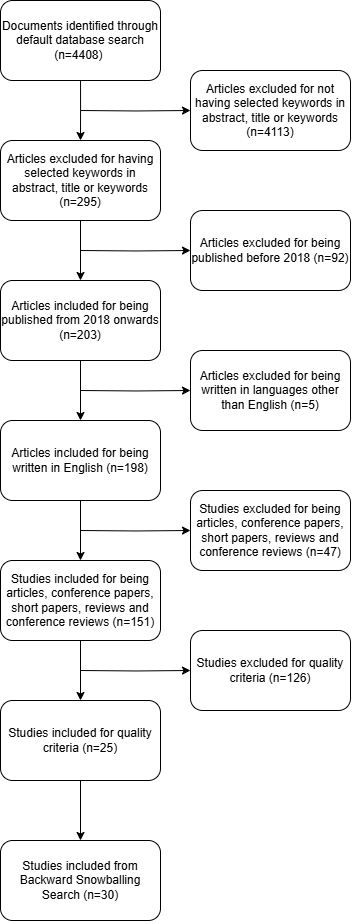
\includegraphics[width=\linewidth, height=0.9\textheight, keepaspectratio]{assets/slr_diagram_backward.png}
    \caption{Flow of the Filtration Process}
    \label{fig:slr_search_filtration_diagram}
\end{figure}
\clearpage
\subsubsection{Data Extraction and Analysis}
\noindent Across the 30 studies selected, most were conference papers (53.3\%) or journal articles (43.3\%), while only 3.3\% of the selected studies were generic articles, as shown in \figref{fig:statistics}. As for the distribution of the studies by publication year, the most predominant year taken into consideration was 2020, with a significance of 33.3\%, followed by 2019 (23.3\%) and 2018 (20.0\%). Together, these three publication years have an importance of more than 75\%, as only 23.4\% of the analyzed studies were published between the years of 2021 and 2023. This may be the case, as the awareness of AGILE and rapid development practices limitations increases, mainly regarding the management of long-term \gls{sq} and the disregard of \gls{nfr} \parencite{Behutiye2020, Melo2022}.


\begin{figure}[htbp]
    \centering
    \begin{subfigure}[b]{0.45\textwidth}
        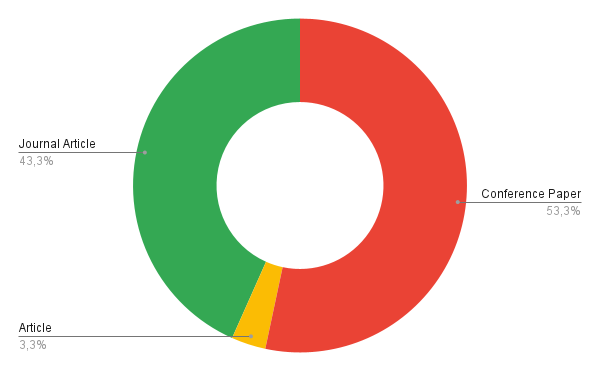
\includegraphics[width=\linewidth]{assets/content_type_chart.png}
        \caption{Distribution of Studies by Content Type}
        \label{fig:content_type_distribution}
    \end{subfigure}
    \hspace{0.05\textwidth} % horizontal spacing
    \begin{subfigure}[b]{0.45\textwidth}
        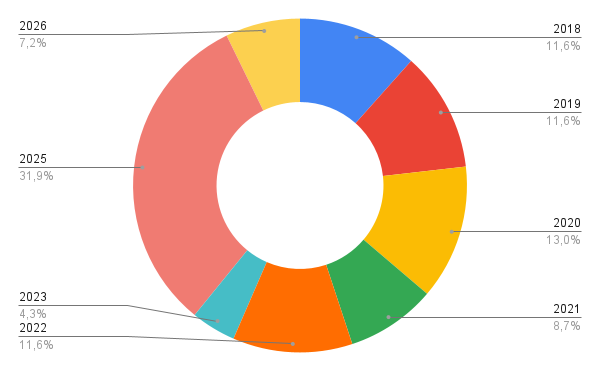
\includegraphics[width=\linewidth]{assets/year_distribution_chart.png}
        \caption{Distribution of Studies by Year}
        \label{fig:year_distribuition}
    \end{subfigure}
    \caption{Statistics}
    \label{fig:statistics}
\end{figure}

\subsection{Review Reporting Stage}
\noindent This section regards the final phase of the \gls{slr} methodology. It encapsulates the extracted data and answers to the outlined research questions. 
\subsubsection{Data Summary}
\noindent To improve the current understanding on the influence of multiple factors of requirements gathering in \gls{td} and \gls{sq}, a collection of key terms utilized in the literature to describe a multitude of concepts regarding \gls{rtd} was determined across the 30 studies. \tabref{tab:key_term_ref} summarizes all the main key term, as well as the number of studies in which each one is used, and the corresponding reference identifiers to those usages. This analysis aims to emphasize both the relevance of certain concepts and the diversity of perspectives and terminologies described across multiple studies.

\begin{table}[htbp]
\centering
\caption{References by Key Terms}
\label{tab:key_term_ref}
\resizebox{\textwidth}{!}{%
\begin{tabular}{|p{5cm}|p{9cm}|r|}
\hline
\textbf{Key Term} & \textbf{References by ID} & \textbf{Total} \\
\hline
Requirements Engineering & S1, S2, S3, S4, S5, S6, S7, S8, S9, S10, S11, S12, S13, S14, S15, S16, S17, S18, S19, S20, S21, S22, S23, S24, S25, S26, S27, S28, S29 & 29 \\
\hline
Technical Debt & S2, S3, S4, S5, S6, S8, S9, S10, S11, S12, S13, S14, S15, S16, S17, S18, S19, S20, S21, S22, S23, S24, S25, S26, S27, S28, S29, S30 & 28 \\
\hline
Evolving Requirements & S23, S27 & 2 \\
\hline
Incomplete Requirements & S8, S17, S24 & 3 \\
\hline
Quality Requirements & S1, S3, S7, S8, S9, S13, S14, S16, S17, S23, S26, S27, S28, S29, S30 & 15 \\
\hline
AGILE & S3, S4, S5, S6, S7, S8, S13, S15, S16, S17, S18, S19, S21, S22, S23, S24, S25, S26, S27, S28 & 20 \\
\hline
Startups & S3, S5, S15, S18, S19, S24, S27 & 7 \\
\hline
Requirement Documentation & S17, S19, S24, S28 & 4 \\
\hline
Non-Functional Requirements & S1, S3, S4, S5, S6, S7, S8, S9, S10, S11, S13, S14, S16, S17, S18, S19, S20, S21, S23, S24, S25, S26, S27, S28, S30 & 25 \\
\hline
Self-Admitted Technical Debt & S1, S2, S9, S11, S12, S14, S17, S19, S20, S24, S30 & 11 \\
\hline
Maintainability & S3, S4, S5, S6, S7, S8, S9, S10, S13, S14, S15, S16, S17, S18, S20, S21, S22, S23, S24, S25, S26, S27, S28, S29, S30 & 25 \\
\hline
Modifiability & S23, S26, S29 & 3 \\
\hline
Scalability & S7, S8, S10, S11, S16, S19, S23, S25, S26, S27, S30 & 11 \\
\hline
Refactoring & S1, S3, S4, S6, S8, S9, S10, S13, S14, S15, S16, S17, S19, S20, S21, S22, S23, S24, S25, S26, S27, S29, S30 & 23 \\
\hline
Preventive Actions & S4, S6, S15, S16, S17, S30 & 6 \\
\hline
Causes Of Technical Debt & S4, S5, S6, S17, S25, S30 & 6 \\
\hline
Mitigation Strategies & S2, S4, S5, S6, S9, S13, S14, S15, S17, S18, S20, S22, S23, S24, S25, S28, S30 & 17 \\
\hline
Requirements Technical Debt & S6, S9, S12, S13, S14, S17, S20, S24, S25, S30 & 10 \\
\hline
\end{tabular}
}
\end{table}
\clearpage
\noindent However, it was also possible to identify several recurring themes regarding the role of requirements gathering and its connection to \gls{td} and \gls{sq}. These were then grouped into four main topics: the Relation of \gls{re} with \gls{sq} and \gls{td}, the Requirement Volatility and Incompleteness as Debt Factors, the AGILE, Startups, and Fast-Paced Development Environments, and the Documentation, Traceability, and \gls{nfr}. Table\ref{tab:main_topics} displays both the number of studies that address each one of the previously mentioned topics and their respective references. 

\begin{table}[htbp]
\centering
\caption{References for Each Main Topic Identified}
\label{tab:main_topics}
\begin{tabular}{|p{7cm}|p{6cm}|c|}
\hline
\textbf{Main Topic} & \textbf{References by ID} & \textbf{Total} \\
\hline
Relation of Requirement Engineering with Software Quality and Technical Debt & S1, S2, S3, S4, S6, S8, S13, S14, S17, S24, S26, S28, S30 & 13 \\
\hline
Requirement Volatility and Incompleteness as Debt Factors & S8, S17, S23, S24, S27 & 5 \\
\hline
AGILE, Startups, and Fast-Paced Development Environments & S3, S4, S5, S6, S15, S18, S19, S24, S25, S27, S28 & 11 \\
\hline
Documentation, Traceability, and Non-Functional Requirements & S1, S3, S7, S9, S10, S11, S13, S16, S17, S24, S28, S30 & 12 \\
\hline
\end{tabular}
\end{table}



\noindent Finally, there was another common ground between the studies in use: the challenges faced by development teams when managing \gls{td} through requirement practices. Five of the main challenges discussed across current literature are: Capturing and Documenting \gls{nfr}, Managing Requirements Volatility and Change, Ensuring Alignment Between Stakeholders and Evolving System Goals, Preventing Long-Term Architectural Degradation through RE Practices, and Refactoring and \gls{td} Mitigation Strategies. \tabref{tab:challenges} outlines the amount of studies in which each of the aforementioned challenges are cited and provides the respective reference identifiers.

\begin{table}[htbp]
\centering
\caption{Challenges Identified in the Literature}
\label{tab:challenges}
\begin{tabular}{|p{7cm}|p{6cm}|c|}
\hline
\textbf{Challenge} & \textbf{References by ID} & \textbf{Total} \\
\hline
Capturing and Documenting Non-Functional Requirements & S1, S3, S6, S7, S8, S9, S10, S14, S17, S18, S24, S28, S30 & 13 \\
\hline
Managing Requirements Volatility and Change & S6, S8, S17, S23, S24, S27 & 6 \\
\hline
Ensuring Alignment Between Stakeholders and Evolving System Goals & S2, S4, S6, S13, S16, S19, S21, S23, S27 & 9 \\
\hline
Preventing Long-Term Architectural Degradation through RE Practices & S3, S4, S5, S13, S14, S15, S17, S25, S26, S30 & 10 \\
\hline
Refactoring and Technical Debt Mitigation Strategies & S1, S4, S6, S9, S13, S17, S20, S22, S23, S25, S28, S30 & 12 \\
\hline
\end{tabular}
\end{table}

\noindent These three tables provided a structured overview of themes explored by current literature. As the data extraction phase aims to provide a deeper understanding of how \gls{re} practices relate to the genesis and mitigation of \gls{td}, the mapping of these dimensions plays a crucial role into providing these insights. 
\subsubsection{Findings Report}
\noindent\textbf{RQ.1}: How do incomplete or evolving requirements contribute to the accumulation of \gls{td} in software development projects?\par

Literature consistently identifies incomplete or mutable requirements as foundational causes of \gls{td}, especially \gls{rtd} \parencite{Melo2022, Waltersdorfer2020}. Throughout the evaluation of current work, it is clear that the end product of projects based on vague, unstable, or weakly-elaborated requirements is often over complicated and flawed at the architecture level.

Both \textcite{Seyff2018, Rios2020} suggest that incomplete requirements often tend to induce developers to make assumptions that bypass formal analysis and validation, resulting in fragile implementations that, in the long-term, create the need to perform code refactoring. Teams resorting to faultier design patterns when \gls{nfr} like performance, security, or usability are not explicitly mentioned in the documentation is an example of this, as it may lead to scalability or maintainability issues later on, as mentioned by \textcite{Farias2020, Wattanakriengkrai2018}, studies in which it is visible how such gaps amplify the likelihood of \gls{satd} - that usually takes form of either comments or workaround code.

AGILE and fast-paced development environments are the main subjects of this issue. As illustrated by \textcite{Gupta2020, Villamizar2018, Vogelsang2020}, changing requirements usually emerge iteratively, and occasionally without sufficient alignment between technical teams. This leads to a snowball effect, where architectural and design choices are reconsidered without adequate planning, incentivizing a reactive development culture, as these constant shifts disrupt the stability of the system's foundations and architecture, which, as the complexity increases, become more complex to refactor.

The solution's security risk is also increased by the absence of traceability \parencite{Rindell2019, Rindell2019b}, as in critical fields such as security, vulnerabilities and long-term maintenance liabilities may be introduced due to misaligned or undocumented requirements shifts.  Additionally, \textcite{Melo2022} highlights that the deficiency of formalized procedures for handling mutable requirements leads to suboptimal prioritization, which then results in codebase embedded trade-offs.

As mentioned by \textcite{Behutiye2022}, changing requirements require appropriate \gls{td} management strategies, as the absence of such approach is likely to compromise system and design integrity. All things considered, the reviewed studies all point to the fact that incomplete and evolving requirements are the perfect conditions for the genesis of \gls{rtd}, that can only be minimized by adopting correct approaches to the problem, such as robust change management, comprehensive \gls{nfr} documentation, and regular requirement validation cycles.



\hspace*{\linewidth}\par
\noindent\textbf{RQ.2}: What is the relationship between the quality of requirement gathering practices and software product quality outcomes over time?\par
Current literature highlights a strong and evident connection between good quality requirement gathering practices and increased software product quality over time \parencite{Femmer2019}. It is suggested that the deployment of methodical, structured \gls{re} practices tend to increase a system's robustness, maintainability, and improves coherence with stakeholder expectations.

\textcite{Behutiye2022} argues that even in settings where documentation is often minimal, such as AGILE, integrating methodic requirement practices enhances the compliance between delivered features and long-term  goals regarding the system architecture, as the amount of misunderstandings and defects can be significantly decreased by applying methods such as the maintenance of lightweight yet complete requirement documentation, stakeholder verification, and version tracking. However, this is not the only author that defends this perspective. In fact, \textcite{Melo2022} goes as far as to support it with evidences, showing that in-depth and well-validated requirements enhances both cross-team communication and the on-boarding of new team members, while also generating records regarding the decision-making process, which all lead to a decreased number of misaligned implementations, which tend to lead to \gls{rtd}.

A connection can also be noted between well-defined requirements and system usability, security, and stability. Recurrent redesigns and regression bugs are usually the result of badly specified requirements - especially \gls{nfr} - as these are in assuring long-term system performance \parencite{Femmer2019}. This is also corroborated by \textcite{Venters2023}, that suggests that system sustainability, which is a metric that covers changeability, performance, and longevity, is a direct consequence of good \gls{re} practices.


\textcite{Vogelsang2020, Siddiqi2020} also emphasize the importance of requirement quality, as they found that low-quality \gls{re} processes forces teams to develop reactively, meaning that issues are only resolved real-world failures or constraints, which increases maintenance costs and also degrades stakeholder trust and decreases the likelihood of further investment.

Moreover, organizations who deploy strong \gls{re} practices are more predisposed to embrace proactive \gls{td} management strategies  \parencite{Waltersdorfer2020}. These organizations also enforce architectural reviews linked to requirement analysis and maintain traceability records linking requirements, tests, and deliveries, leading to a decreased ambiguity and allowing teams to be more effective at  refactoring.

At last, current work indicates that \gls{re} quality is a deeply tied to \gls{sq}. By utilizing proper documentation, stakeholder involvement, traceability, and iterative validation, requirement gathering practices lead development towards more consistent, scalable, and maintainable solutions, while increasing their quality.

\hspace*{\linewidth}\par
\noindent\textbf{RQ.3}: Which requirement-related factors most commonly lead to \gls{td}, and how are they identified and mitigated in practice?

\gls{rtd} manifests as an ongoing, multi-dimensional challenge in the literature, largely caused by a composition between structural weaknesses during the \gls{re} process and organizational practices that lack emphasis on long-term maintainability \parencite{Melo2022}. While it is true that \gls{rtd} may be dependent on multiple variables, that can independently or collectively increase it, current work systematically emphasizes a pattern in the underlying causes, along with practical methods to both identify and mitigate \gls{rtd}.

One of the main causes of \gls{rtd} is the lack of proper specification and documentation of \gls{nfr}. Teams usually tend to primarily focus functional aspects due to time-critical deadlines, thus overlooking critical quality aspects such as product performance, security, and scalability \parencite{Farias2020, Behutiye2022}, which has consequences, as the system evolution continues without structural architecture planning required to fulfill these expectations, meaning that deliveries end up architecturally fragile and employing quick fixes that reflect accumulated debt rather than intentional design.


An aggravating factor to this problematic is the absence of traceability and useful documentation, as mentioned by \textcite{Rios2020, Wattanakriengkrai2019}. According to the authors, the decentralization of requirement sources, varying from informal meetings to dispersed documentation tools, is a pivotal element in decreasing consistency, as teams cannot confidently asses the impact certain implementation might have when changes or the reasoning behind certain decisions are not recorded. This leads to the build up of uncertainty, that subsequently encourages design decisions that emphasize short-term results rather than architectural stability.

The nonalignment between business stakeholders and development teams also leads to the accumulation of \gls{rtd}; current work shows that the failure to establish communication between the aforementioned actors tends to result in divergent understandings of what a requirement includes. Business needs are prone to swiftly evolving or shift priorities, but without a shared vision, empowered by structured debates or shared artifacts,  development teams can utilize outdated or unfinished requirements, resulting in misaligned implementations that are noticeable after their execution, when the cost of refactoring is increasingly bigger than the cost of correctly implementing the correct approach from the get go \parencite{Seyff2018, Gralha2018}.

Another regularly verified problem is the pace at which requirements progress without adequate architectural revision. Although iterative and AGILE methodologies embrace change, current work alerts for the risk that constant iteration, without well-planned refactoring, poses, as it inputs systemic misalignment between the initial design and its implementation. This is demonstrated by \textcite{Rindell2019} in respect to security-related features, and how not updating threat models or re-validating architectural assumptions when trying to adapt to evolving business needs compromised projects. Similarly, \textcite{Villamizar2018} proposes that  requirement volatility requires the presence of thorough change management, in order to prevent the dissemination of underlying debt across related modules.

The deviation between \gls{re} practices and subsequent technical processes also contributes to the accumulation of \gls{rtd}. When requirement specification documents are not seamlessly unified with design, testing, and deployment streams, an increase on deficiencies is noticed, yet, they are not flagged until late stages of the development lifecycle. According  to \textcite{Venters2023}, the absence of alignment previously mentioned obstructs the organization from a holistic perspective on system quality, constraining their capacity to preemptively address problems.

Current literature suggests a range of mitigation and identification strategies regarding these challenges. Examples of this are the use of automated tools to detect \gls{satd} within codebases by analyzing comments and commit messages that may display signs of requirement deviations \parencite{Li2020} or the  deployment of frameworks dedicated to assess the requirement health, such as those by mentioned by \textcite{Lenarduzzi2019}, which present metrics to evaluate the completeness, clarity, and stability of requirement artifacts. Another possible strategy to identify the described challenges is the implementation of bidirectional traceability systems, that enable early the detection of requirement violations and better impact analysis upon change introduction \parencite{Siddiqi2020}.

Integrating mitigation approaches in development team culture and workflows is beneficial, as performing frequent stakeholder meetings, recursive refinement of requirement documents, and the inclusion of \gls{re} reviews in sprint retrospectives all lead to less \gls{rtd} build-up. \textcite{Rios2020} suggests that the integration of \gls{re} practices into AGILE ceremonies, such as backlog refinements and sprint reviews, helps on the early recognition and remediation of requirements-related issues that impact product quality. Finally, existing research supports the utilization of explicit debt trackers, in which identified \gls{rtd} occurrences must be documented, prioritized, and prepared for rectification \parencite{Melo2022}.

In conclusion, requirement-related variables that contribute to \gls{td} are highly correlated with both technical approaches and organizational culture. The incidence and severity of \gls{rtd} can be decreases by fostering requirement clarity, traceability, and integrating \gls{re} with technical processes, and criticality of \gls{rtd}. \textcite{Melo2022} emphasizes that ambiguous, poorly specified, untraceable requirement tend to make software deliveries more prone to refactoring and architecture degradation The author also mentions that well-established practices for the governance leads teams to face less long-term quality issues.

\hspace*{\linewidth}\par
\noindent\textbf{RQ.4}: 
What \gls{re} process is most commonly linked to \gls{td}, and how can they improve to mitigate it?\par

Across the analysed literature, the accumulation of \gls{td} is commonly associated with AGILE and fast-paced 
environments, largely due to the pressure associated with these environments and with how requirements are handled 
under pressure. \textcite{Behutiye2020} highlights that \gls{qr} are usually deprioritized over \gls{fr}, which 
leads to the underdocumentation of \gls{qr}, while also states that \gls{td} in AGILE Software Development is often 
generated by inadequate or missing knowledge of \gls{qr} and \gls{fr}.

Besides this, due to its focus being continuos delivery, AGILE Software Development is more prone to 
\gls{td} accumulation than traditional software development \parencite{Rios2019}.

When tackling the situation from a processual standpoint, the recurring option is to strengthen \gls{re} in AGILE 
environments with concrete practices and artifacts that revolve focus on the solution's architecture and 
\gls{qr}, while still not compromising AGILE's characteristic iterative nature when creating deliverables,
as \textcite{Snoeck2022} argue that \gls{td} is often caused by the lack of architectural thinking associated with 
AGILE, and propose an integrated method that enables a decrease of \gls{td} by engineering the architecture in a 
logical, consistent and complete manner.

\gls{re} processes can be improved by highlighting \gls{td} and \gls{rtd} and by improving the workflow to introduce governance practices, 
in order to avoid reactive prioritization, as \textcite{Besker2019} report that \gls{td} prioritization is commonly 
reactively and lacks the usage of specific strategies and that \gls{td} items are often managed and 
prioritized in an alternative backlog.
In conclusion, current literature consistently correlates AGILE/fast-paced contexts to \gls{td} through \gls{qr} 
neglect, as well as frail documentation and reactive handling of \gls{td}, while the improvements mentioned are the 
reinforcement of AGILE \gls{re} practices with explicit \gls{qr} and architecture practices, as well as the 
integration of the backlogs in which \gls{td} is tracked into the main backlog of the development teams.



\hspace*{\linewidth}\par
\noindent\textbf{RQ.5}: 
How do different project contexts and team structures affect the emergence or management of \gls{rtd}?\par

\gls{rtd}'s existence is strongly dependant on the project's technical and social context, especially on the 
organizational constraints, stakeholder fragmentation, and on the degree of cross-team awareness over 
dependencies. In complex, industrial settings, the automotive development is, according to \textcite{Vogelsang2020}, 
extremely influenced by legacy systems and organizational constraints, as well as OEM/supplier relationships, which 
worsens the coordination and generates challenges regarding \gls{re}. \textcite{Vogelsang2020} also notes that these 
contexts are favorable for \gls{rtd}-relevant dependencies to remain imperceptible, reinforcing that a team's
structure and the way knowledge is distributed are directly related to how early requirement-linked issues are 
detected. In multi-stakeholder environments with various artifacts, the validation and 
verification of exchanged artifacts  becomes, according to \textcite{Waltersdorfer2020}, "cumbersome and error-prone”. 
This, of course, increases the risk of mismatches between requirements and real implementation.

However, \gls{rtd} management is not just a technical problem - there is also a interpersonal and organizational 
dimention to it - which \textcite{Melo2022} conclude is not properly addressed. 
Overall, the literature converges on the idea that larger or more heterogeneous projects, with legacy constraints, multiple stakeholders, and fragmented tooling,
are more prone to \gls{rtd} and are harder to proactively manage. Besides this, having teams with limited awareness of dependencies and weak cross-stakeholder 
validation also increase the likelyhood of late discovery and costly remediation of \gls{rtd}.

\subsection{\gls{slr} Conclusions}

This \gls{slr} investigated the link between \gls{re} and \gls{td}, particularly focusing on the causes and of effects of \gls{rtd}. Throughout all 30 analyzed studies, it becomes evident that the quality and management of requirements are key factors when analyzing the success and quality of a  software system.

A key insight that can be extracted by this study is that incomplete or ever-changing requirements have a very meaningful impact on the compounding of \gls{td}. Regardless of the development philosophy, wether it is AGILE or a more traditional development context, the failure to solidly identify or iteratively validate requirement is strongly linked to the development of fragile architectures, heavy refactoring costs and to the need for long-term maintenance. The research also implies that reactive development practices, in which there is no update to neither the documentation nor to the architecture when accommodating unforeseen changes, are especially harmful, as they build-up over time and blur the original goals of the system.

Another key factor to mention is the impact that requirement gathering quality has in it comes to the quality of software deliverables. Requirement practices  that involve stakeholders, thorough documentation, and traceability, are linked to higher-quality software, as solutions are more likely to be more maintainable, scalable, and user-aligned. Contrarily, informal or fragmented \gls{re} processes are heavily linked to miscommunication between developer and business teams, misalignment between deliverables and stakeholder expectations, and improvised development decisions, which are a breeding ground for \gls{rtd}. Current work supports the argument that investing in good practices of \gls{re} early on results in lasting advantages in \gls{sq} and cost-efficiency.

This study also unveils requirement-related variables that increase \gls{td}: it stresses the risk of overlooking \gls{nfr}, undocumented changes, and communication gaps between business and technical standpoints. Both cultural and technical shifts are necessary to address these issues. Processes such as \gls{satd} detection, requirement traceability, the involvement of stakeholders in the elaboration of requirement artifacts, and the upkeep of explicit \gls{td} repositories represent concrete methods teams can use to abandon reactive \gls{td} management in favor of a more proactive approach.

Collectively, the outcomes of this review have both academic value and real world applications. As for professionals, the study aims to unequivocally position \gls{re} as more than just a preliminary phase of development. This process must be everlasting and evolve alongside the system. For the academy, the review points out research gaps, such as the limited focus on proactive \gls{rtd} prevention and the influence of organizational culture on \gls{rtd} build-up. \gls{nfr} and domain-specific contexts, such as safety-critical systems, for instance, are also underdeveloped. Future research should focus on developing and deployed prevention frameworks, researching team and organizational variables, and improving \gls{nfr} management to reduce long-term cost and respective debt.

In conclusion, this review reinforces that \gls{td} is a controllable outcome of intentional design decisions, rather than an inevitable effect of fast-paced development. By treating requirements with the necessary rigor and strategic attention they require, development teams are enabled to create systems that are not only functional, but also sustainable.

\section{Multivocal Literature Review}
\noindent In addition to the \gls{slr}, a \gls{mlr} was also conducted, complementing the findings previously obtained from academic literature with grey literature sources, so that more practical perspectives can also be taken into consideration, as the software engineering industry is in constant evolution, and new practices, tools and frameworks are frequently adopted by teams in this industry \parencite{Garousi2019}. The \gls{mlr} aims to capture insights that may not still be presented in academic publications (and, therefore, that might have not been captured by the previous \gls{slr}), thus providing a more well-rounded view of the relationship between \gls{re} and \gls{td} and what are the practices utilized in the real world to handle this subject. Another goal of this MLR was to also provide better comprehension on how the industry currently defines \gls{td} and how requirements engineering processes have been adapted over time to better tackle \gls{td} management.
In order to conduct the \gls{mlr}, the search string was tweaked, so that it matches the exact goal of this literature review - represented on \tabref{tab:mlr_search_string}. Pieces of grey literature were also filtered by selection criteria previously defined, displayed in \tabref{tab:mlr_filters}.

\begin{table}[htbp]
    \centering
    \begin{tabular}{|>{\columncolor{gray!30}}c|c|}
        \hline
        Search String & ""Requirement" AND "Technical" AND "Debt" in "Software""\\
        \hline
    \end{tabular}
    \caption{MLR Search string}
    \label{tab:mlr_search_string}
\end{table}

\begin{table}[htbp]
    \centering
    \begin{tabular}{|c|c|}
        \hline
        \rowcolor{gray!30}
        ID & Filter \\
        \hline
        1 & Must be relevant for the study research \\
        \hline
        2 & English \\
        \hline
        3 & Source must be trusted \\
        \hline
    \end{tabular}
    \caption{Search Filters}
    \label{tab:mlr_filters}
\end{table}

\chapter{Research Methodology}
This study follows a mixed approach based in \gls{dsr}, which, according to \textcite{Brocke2020}, is a
 “a problem-solving paradigm that seeks to enhance human knowledge via the creation of innovative
  artifacts”. However, as the study strives to output both an artifact while also an explanation for a real-world phenomenon,
  it also integrates \gls{csr}, which can be used “before the 
  design of the artifact… to evaluate some preliminary forms or some parts of 
  the artifact” \parencite{Costa2016}.

\section{Design Science Research}
\gls{dsr} sets the foundation this dissertation. As described by \parencite{Brocke2020}, \gls{dsr}
is “a problem-solving paradigm that seeks to enhance human knowledge via 
the creation of innovative artifacts”, which has as its main goal to “extend the 
boundaries of human and organizational capabilities by designing new 
and innovative artifacts” \parencite{Brocke2020}.

In order to apply this methodology, the problem must be identified, 
as well as solution objectives, which will lead to the design and 
development of the final artifact, which will then be demonstrated, 
evaluated, and communicated \parencite{Brocke2020}, displayed in \figref{fig:dsr_phases}.

\begin{figure}[htbp]
    \centering
    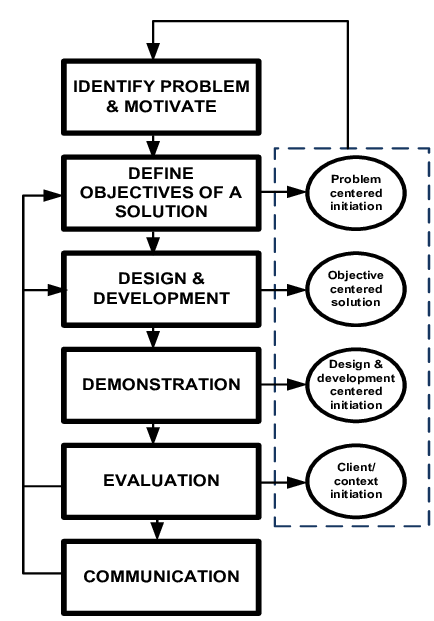
\includegraphics[width=0.4\textwidth]{assets/dsr_methodology_flow_chart.png}
    \caption{Design Science Research Phases}
    \label{fig:dsr_phases}
\end{figure}

\section{Case Study}
\noindent The study also implements a case study methodology, outlined by \textcite{Runeson2009}, to explore the impact of \gls{re} practices on \gls{rtd} in a corporate context. The purpose of this case study is to identify and scrutinize how real-world software development teams within the studied company approaches \gls{re} and \gls{rtd} in daily workflows.

The study will collect data by means of interviews, document analysis, and monitoring of project artifacts and sprint ceremonies. Insights will be triangulated in order to comprehend how \gls{td} accumulation is impacted by requirement quality, documentation, and traceability. The findings will be evaluated relative to the outcomes of the \gls{slr} to validate, contrast, and extend established knowledge. In conclusion, the study seeks to contribute to the generation of relevant, customized suggestions for improving \gls{re} practices in the company.

\begin{figure}[htbp]
    \centering
    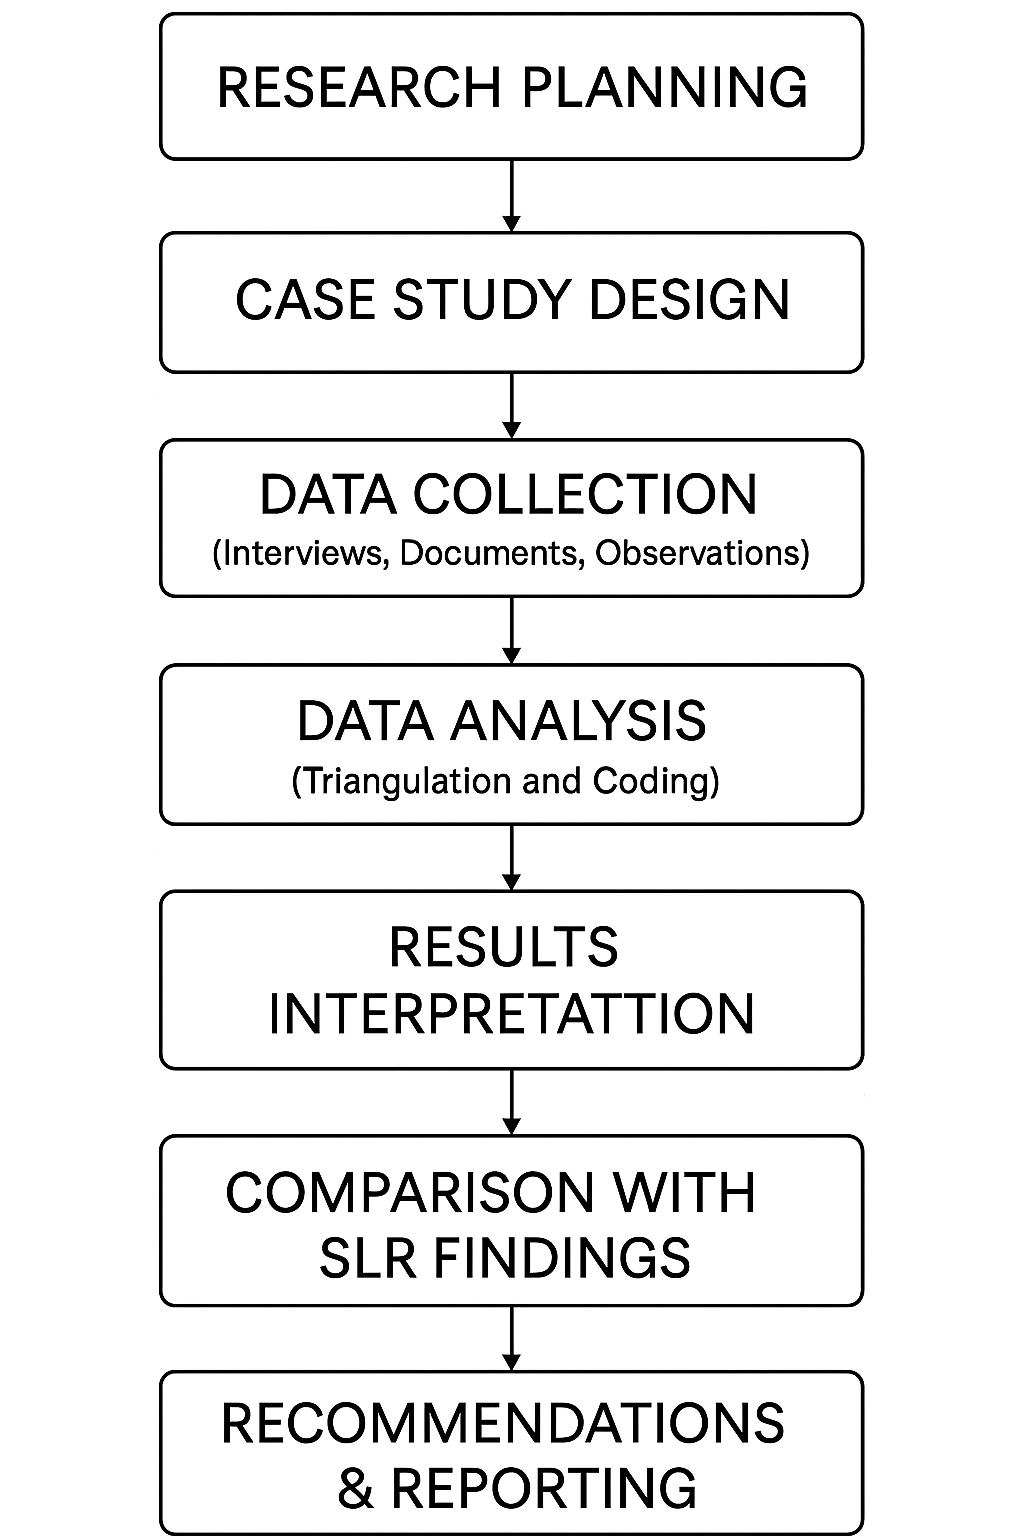
\includegraphics[width=0.4\textwidth]{assets/case_study_flow_diagram.png}
    \caption{Case Study Elaboration Phases}
    \label{fig:case_study_phases}
\end{figure}

\section{Hybrid Methodology}
\noindent The methodological design of this dissertation combines 
\gls{dsr} and \gls{csr}. This mixed approach is adopted in order to both analyse an empirical 
phenomenon and develop an artifact, as \textcite{Costa2016} emphasizes that \gls{csr} provides 
essential “knowledge about the empirical context”, enabling a better and more precise definition of the 
problem, stakeholders, and requirements for the artifact in development. 

This supports \textit{ex-ante} activities, such as refining objectives and grounding design decisions in real organizational practices.

\textcite{Nabukenya2012} reiterates the value of utilized an hybrid methodology, arguing that “combining \gls{csr}, 
\gls{dsr} and AR methods is most suitable to support the execution” of research closely tied organizational practices. 

Together, the merger of these two methodologies creates a coherent research strategy that promotes precision, contextual relevance, practical utility and ensures that the most current industry practices are being taken into consideration.
\begin{figure}[htbp]
    \centering
    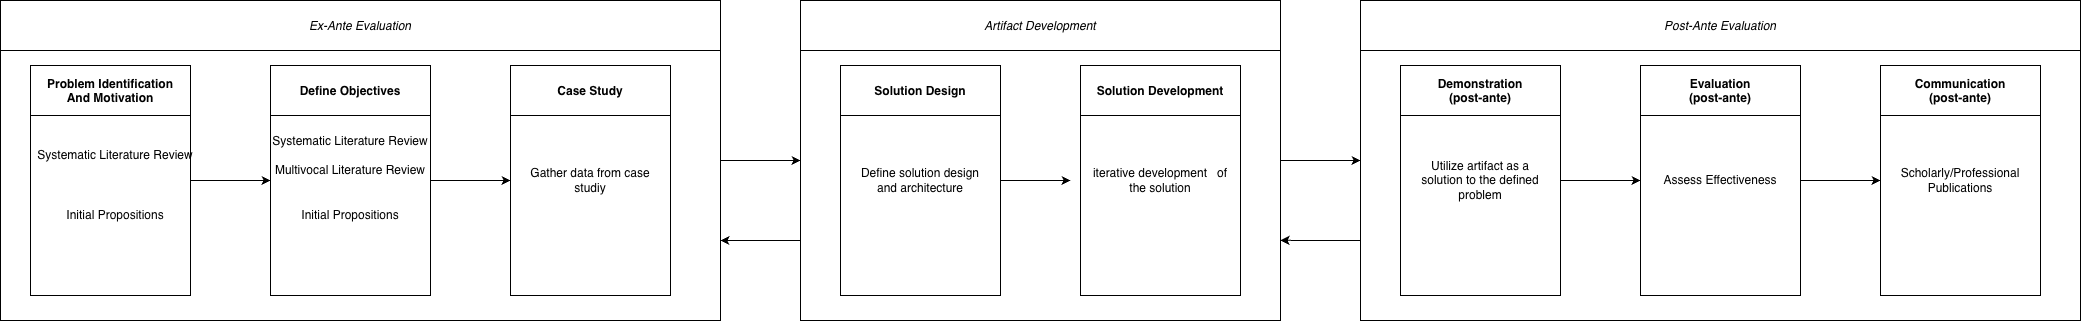
\includegraphics[width=1\textwidth]{assets/research_methodology_flow_chart.png}
    \caption{Research Methodology Phases}
    \label{fig:research_methodology_phases}
\end{figure}

\renewcommand{\bibname}{References}

\printbibliography

\clearpage
\appendix
\renewcommand{\thefigure}{\thechapter.\arabic{figure}}
\begin{landscape}
\begin{center}
\small
\renewcommand{\arraystretch}{1.1}
\begin{longtable}{|c|p{5cm}|p{4.5cm}|c|c|p{5.5cm}|}
\hline
\textbf{ID} & \textbf{Title} & \textbf{Authors} & \textbf{Year} & \textbf{Type} & \textbf{Source} \\
\hline
\endfirsthead
\hline
\textbf{ID} & \textbf{Title} & \textbf{Authors} & \textbf{Year} & \textbf{Type} & \textbf{Source} \\
\hline
\endhead
\hline
\endfoot
\hline
\endlastfoot
S1 & Actions and Impediments for Technical Debt Prevention: Results From a Global Family of Industrial Surveys & \citeauthor{Freire2020} & 2020 & Conference Paper & Proceedings of the 35th Annual ACM Symposium on Applied Computing \\
S2 & A Longitudinal Study of Identifying and Paying Down Architecture Debt & \citeauthor{Nayebi2019} & 2019 & Conference Paper & ICSE-SEIP \\
S3 & AGILE MERODE: A Model-Driven Software Engineering Method & \citeauthor{Snoeck2022} & 2022 & Journal Article & Software and Systems Modeling \\
S4 & Automatic Classifying Self-Admitted Technical Debt Using N-Gram IDF & \citeauthor{Wattanakriengkrai2019} & 2019 & Conference Paper & APSEC \\
S5 & Causes and Effects of the Presence of Technical Debt in AGILE Projects & \citeauthor{Rios2019} & 2019 & Conference Paper & SEAA \\
S6 & Crowd-Focused Semi-Automated Requirements Engineering & \citeauthor{Seyff2018} & 2018 & Conference Paper & IEEE RE \\
S7 & Experiences With Technical Debt and With Its Management Strategies in Practice & \citeauthor{Waltersdorfer2020} & 2020 & Conference Paper & TechDebt \\
S8 & Feature Dependencies in Automotive Software Systems: A Multi-Method Study & \citeauthor{Vogelsang2020} & 2020 & Journal Article & Journal of Systems and Software \\
S9 & Fostering Continuous Value Proposition Innovation Through Freelancer Involvement: An Action Design Research Approach & \citeauthor{Gupta2020} & 2020 & Journal Article & Sustainability \\
S10 & Hearing the Voice of Software Practitioners on Documentation Debt: A Mapping Study & \citeauthor{Rios2020} & 2020 & Book Chapter & LNCS \\
S11 & Identification and Remediation of Self-Admitted Technical Debt in Issue Trackers & \citeauthor{Li2020} & 2020 & Conference Paper & SEAA \\
S12 & Identifying Design and Requirement Self-Admitted Technical Debt Using N-Gram IDF & \citeauthor{Wattanakriengkrai2018} & 2018 & Conference Paper & IWESEP \\
S13 & Identifying Self-Admitted Technical Debt Through Comment Analysis Using Contextual Vocabulary & \citeauthor{Farias2020} & 2020 & Journal Article & Information and Software Technology \\
S14 & IMDfence: Architecting a Secure Protocol for Implantable Medical Devices & \citeauthor{Siddiqi2020} & 2020 & Journal Article & IEEE Access \\
S15 & Interdisciplinary Effects of Technical Debt in Companies With Mechatronic Products & \citeauthor{Vogel-Heuser2021} & 2021 & Journal Article & Journal of Systems and Software \\
S16 & Is Using Deep Learning Frameworks Free? Measuring the Cost of DL Frameworks From a Technical Debt Perspective & \citeauthor{Liu2020} & 2020 & Conference Paper & ICSE-SEIS \\
S17 & Managing Security in Software: Or: How I Learned to Stop Worrying and Manage the Security Technical Debt & \citeauthor{Rindell2019} & 2019 & Conference Paper & ARES \\
S18 & On the Relationship Between Technical Debt Management and Process Models: A Case Study of a Start-Up Company & \citeauthor{Rios2021} & 2021 & Journal Article & IEEE Software \\
S19 & Requirements Quality is Quality in Use & \citeauthor{Femmer2019} & 2019 & Journal Article & IEEE Software \\
S20 & Security Risk Assessment and Management as Technical Debt & \citeauthor{Rindell2019b} & 2019 & Conference Paper & Cyber Security Conference \\
S21 & Software Sustainability: Research and Practice From a Software Architecture Viewpoint & \citeauthor{Venters2018} & 2018 & Journal Article & Journal of Systems and Software \\
S22 & Sustainable Software Engineering: Reflections on Advances in Research and Practice & \citeauthor{Venters2023} & 2023 & Journal Article & Information and Software Technology \\
S23 & Technical Debt Triage in Backlog Management: An Industrial Case Study & \citeauthor{Besker2019} & 2019 & Conference Paper & TechDebt \\
S24 & The Evolution of Requirements Practices in Software Startups: A Grounded Theory of AGILE and Flexible Development & \citeauthor{Gralha2018} & 2018 & Conference Paper & ICSE \\
S25 & Towards a Holistic Definition of Requirements Debt & \citeauthor{Lenarduzzi2019} & 2019 & Conference Paper & ESEM \\
S26 & Towards Optimal Quality Requirements Documentation in AGILE Software Development & \citeauthor{Behutiye2022} & 2022 & Journal Article & Journal of Systems and Software \\
S27 & A Systematic Mapping Study on Security in AGILE Requirements Engineering & \citeauthor{Villamizar2018} & 2018 & Conference Paper & SEAA \\
S28 & Automatic Identification of Self-Admitted Technical Debt From Four Different Sources & \citeauthor{Li2023} & 2023 & Journal Article & Empirical Software Engineering \\
S29 & Identification and Measurement of Requirements Technical Debt: A Case Study in a Large-Scale AGILE Environment & \citeauthor{Melo2022} & 2022 & Journal Article & Journal of Systems and Software \\
S30 & Is Using Deep Learning Frameworks Free? Characterizing Technical Debt in Deep Learning Frameworks & \citeauthor{Liu2020} & 2020 & Conference Paper & ICSE-SEIS \\
\end{longtable}
\end{center}
\end{landscape}


\end{document}
